\chapter{Theoretical Framework}\label{ch1:Intro}

\section{Hydrogels}

\paragraph{Introduction} From bibliographic review, we can say that a hydrogel is a polymeric network that has the capacity of swelling[cites].
Some examples are,
    polyacrylamide,
    sodium polyacrylate,
    Poly(vinyl alcohol),
    Poly(ethylene glycol),
    Poly(hydroxyyethyl methacrylate),
    agarose,
    alginate,
    gelatin,
    pectin,
    starch,
    cellulose-based networks,
    protein networks,
    among others.
In order to try to understand (some of) the properties of the hydrogels, we are going to explore what is a polymeric network and what is the capacity of swelling.

In general terms, a polymeric network is a three dimensional structure formed by long polymer chains that are interconnected.
Meanwhile, the swellability is defined as the capacity to absorb significant amounts of a solvent without dissolving, resulting in an increase volume.
Since the swellability is a ``capacity'' of the network, we are going to start by exploring what is a polymeric structure.

\subsection{Polymeric networks}

\paragraph{Introduction} From a structural perspective, polymer networks consist of network ``junctions'', which consist of three or more strands connected by a mechanism. 
This mechanism is commonly refer as ``crosslink'' and can be describe through physical interactions or covalent bonds.
On the other hand, we recall that a polymer is a macromolecule composed by monomers that are covalently bondend together forming a strand.
Monomers can possess specific functional groups or reactive sites, which determine the manner in which monomers bind together. 
This, in turn, influences the structural and property characteristics of the resulting polymer.
Part of the swelling capacity can be explained by the type of monomers in the network, meanwhile the structural frameworks allows to explain the mechanical response and the swelling.

\paragraph{Swellability} The capacity for substantial solvent absorption and expansion of hydrogels is attributable to the expansion of the network due to osmotic pressure and the hydrophilic funcional groups of the monomers that constitute hydrogels.
Some of the key hydrophilic groups are,
    hydroxyl group,
    amide group,
    carboxylate anion,
    ether group.
The hydrophilic phenomenon, from a chemical perspective, occurs when molecules possess polar or charged functional groups that spontaneously form hydrogen bonds or electrostatic interactions with water, enabling water to diffuse over the surface.
Nevertheless, the network's integrity remains intact due to the crosslink mechanism.

\paragraph{Crosslink} The underlying principles of crosslink mechanism are the physical interactions and covalent bonds.
However it is important to acknolwdge that, for example, given sufficiently strong and static physical interactions, physical networks can behave identically to covalent bonded networks; 
alternatively, the incorporation of mechanisms for covalent bond exchange can result in chemical networks that exhibit adaptable mechanical properties regulated by external stimuli [cite]. 
Consequently, an emphasis on bond strengths and exchange rates provides more informative insights for accurately inferring the properties of hydrogels.

With this understanding, a covalent bond is defined as a specific type of chemical bond that occurs when two atoms share one or more pairs of electrons. 
On the other hand, a physical interaction is defined as a non-covalent force that describes how atoms, ions, or molecules attract or repel each other without forming new chemical entities. 
The covalent bond is the result of quantum mechanical interactions between atomic orbitals.
In these interactions, shared electrons occupy a molecular orbital that extends over both atoms. 
In contrast, physical interactions are attributed to electrostatic, van der Waals, or dipole forces, arising from the redistribution of electron density and the consequent energy alterations between particles.

Now we can dive into the different types of polymer networks and the different types of crosslink mechanisms.
After that, then we are going to spend some paragraphs into explore the ideas of mechanical response through constitutive relations.
In order to end with the mechanical response of hydrogels and some conections with the polymeric network.

\subsection{Types of polymeric networks: Gels}

\paragraph{Introduction} In general terms a polymeric network can be divided into one of four major classes: 
    thermosets,
    thermoplastics,
    elastomers,
    and gels.
Thermosets are rigid, covalently bonded polymer networks with high modulus, which are insoluble and degrade rather than melt upon heating. 
In contrast, thermoplastics are held together by strong physical interactions, allowing them to be remolded and recycled when heated. 
Elastomers are soft, deformable with covalent networks used above their glass transition temperature, capable of large reversible extensions. 
Finally, gels are liquid-swollen networks, either covalent or physical interactions, that are soft and highly deformable.

\paragraph{Gels} In detail, a gel is a three-dimensional, crosslinked polymer network formed by physical or chemical crosslinks, which serve to trap the solvent molecules via intermolecular interactions, including hydrogen bonding and osmotic forces. This process prevents the fluid from flowing freely.
This results in a material with both solid and liquid characteristics—elasticity from the polymer network and fluidity from the entrapped solvent.
This description resembles that of a hydrogel.
The hydrogel, however, is a specific type of gel in which the solvent is water and the polymers are hydrophilic.

\paragraph{Gel point} The classification of a polymer network as a gel is characterized by the formation of a continuous, system-spanning (infinite) network through the process of polymerization or crosslinking mechanisms.
This phenomenon is indicative of the percolation\footnote{In physics, percolation describes the emergence of large-scale connectivity in disordered systems. On the other hand, mathematically, is the study of cluster formation in a random graph or lattice when sites or bonds are occupied with a given probability.} of the polymeric network.
And it is known as the gel point.
At this point, the polymer chains become sufficiently interconnected through crosslinks to create a macroscopic network that spans the entire volume, causing the material to gain elasticity and lose fluidity, transitionning\footnote{This transition is a percolation threshold where the molecular weight and network correlation length diverge.} it from a viscous liquid (sol) to a solid-like gel.

Finally, it must be mentioned that not all polymer networks can achieve a gel point.
To reach this point requires sufficient network connectivity due to enough reactive sites and a high enough crosslinking density.
For instance, linear, unbranched, or insufficiently crosslinked polymers remain soluble and do not gel.

\subsection{Crosslink mechanisms}

\paragraph{Intro} According to the literature, the most common classification is typically as physical or covalent hydrogels.
In regards to the main crosslink mechanism present in the polymeric network.
However, it is important to note that, although the crosslink mechanism plays a significant role in network integrity, it is not the sole mechanism that can adequately describe the mechanical response in terms of network structure.
In this regard, three primary crosslink mechanisms can be identified: covalent, physical interactions, and mechanical\footnote{No estoy seguro si hablar de técincas de sintetización o si explicar mejor los mecanismos de bond exchange en redes covalentes y en redes físicas.}.

\paragraph{Covalent Crosslinking} Polymer chains are linked by covalent bonds, which are typically formed through free-radical polymerization, click chemistry, or UV-induced reactions.
This results in a static, stable, and robust network with high mechanical strength and low reversibility.
However, when dynamic covalent chemistry is applied, it can allow bond exchange and self-healing properties.

\paragraph{Physical Crosslinking} Polymer chains are held together by non-covalent interactions, including hydrogen bonding, ionic interactions, hydrophobic associations, and van der Waals forces.
Given the possibility of bond exchange under normal conditions, the network is dynamic.
Therefore, they tend to be softer and less mechanically robust in comparison to covalently crosslinked hydrogels.
Finally, these networks are reversible, enabling self-healing, shape-memory, and stimuli-responsive behaviors.

\paragraph{Mechanical Crosslinking} Finally, these types of crosslinked networks are held together by physical entanglements or interpenetrating polymer chains.
Examples include double-network hydrogels, slide-ring gels, and highly entangled architectures.
This provides toughness and elasticity properties by dissipating energy through chain movement and entanglement.

\subsection{Reverible networks}

\paragraph{Intro} Another common classification in literature is to categorize the polymeric network as reversible or irreversible.
It is a common association that networks with physical crosslink mechanisms are reversible, while covalently crosslinked networks are irreversible.
However, regardless of the crosslink mechanism, the network can be shown to be reversible.

\paragraph{Physical networks} The interactions can spontaneously break and reform due to thermal fluctuations or changes in the microenviroment, sucha pH, ionic strength, temperature.
When external stress or energy disturbs the network, some physical bonds dissociate. 
Free chain segments then seek new partners, allowing dynamic rejoining at different sites. 
This ongoing exchange can lead to self-healing, viscoelastic behavior, and adaptability of the hydrogel.
The equilibrium and kinetics of bond formation/dissociation can be tuned by controlling the physical interactions.

\paragraph{Covalent networks} In ``dynamic'' covalent bonds, such as imine, boronate ester, thioester, disulfide, and transesterification, the network has the capacity to break and reform via chemical equilibrium. 
This process is driven by external stimuli, including temperature, pH, or catalysts.
The external stimuli facilitate the exchange of polymer chains at crosslinked points through either associative or dissociative mechanisms.
The associative mechanism occurs when new bonds form before old bonds break. In contrast, the dissociative mechanism occurs when old bonds break before new bonds form.
The exchange of polymer chains enables the material to exhibit self-healing, stress relaxation, and shape adaptability while maintaining the mechanical strength provided by covalent bonds to the network.
Finally, it is important to note that the energy barrier for exchange, bond stability, and stimulus-dependence govern the rate and reversibility of the process.


\section{Mechanical response}


\marginpar{In the following methodology, we will couple the macroscopic and microscopic scale:
    We employ the macroscopic constitutive relations; however, the stress tensor is defined from the microscopic scale.

\begin{gather}
    \epsilon_{ij} = \frac{1}{2}\left( \pdv{u_i}{x_j}+\pdv{u_j}{x_i} \right)\label{eqn:strainTensor}
\end{gather}
This mathematical representation is only valid for infinitesimal small deformations.
Where $u_i$ are the component of the displacement vector field and $x_j$ are the spatial coordinates.
}

\begin{comment}
\begin{gather}
    \vec{T} = \bm{\sigma}\cdot\vec{n}\label{eqn:stressTensor}
\end{gather}
where the operation of the dot product between the normal vector with a tensor is 
\begin{gather*}
    \begin{bmatrix}
        \sigma_{11} & \sigma_{21} & \sigma_{31} \\
        \sigma_{12} & \sigma_{22} & \sigma_{32} \\
        \sigma_{13} & \sigma_{23} & \sigma_{33} \\
    \end{bmatrix}
    \cdot
    \begin{bmatrix} n_1 & n_2 & n_3 \end{bmatrix}.
\end{gather*}
The component $\sigma_{ij}$ represents the force in the $i$-th direction acting on a surface perpendicular to the $j$-th coordinate axis.
Also, the tenso is symmetric under the usual ssumption of no body torques and balance of angular momentum.
\end{comment}

The concept of a material's mechanical response describes the relationship between the deformation of a material and the applied stress and/or shear rate.
Nevertheless, this relationship can be described from a macroscopic scale and also from a microscopic scale.
At the macroscopic level, the description captures the effective mechanical response as a continuum property. 
At the microscopic level, it provides insights into the origin of the mechanical response and how structural features at small scales control the macroscopic response.
In this section, we will delve into the various descriptions and explore the quantification of this relationship.

\paragraph{Constitutive relations} The relationship between deformation and stress is expressed through a constitutive equation.
This equation is a mathematical tool that quantifies the relationship. 
It is used to predict or model material behavior, as reflected by empirical observations.
Additionally, these equations can be defined from both the microscopic and microscopic scale.
These two scales are linked through the implementation of averaging or homogenization procedures.
However, there is a difference in interpretation and application.
Thse issues will be addressed in the following sections.

\paragraph{Tensors} Before proceeding, it is necessary to know the quantitative representation of stress and strain.
Both quantities are mathematically represented as second-rank tensors, which can be algebraically expressed as a $n\times n$ matrix.
Furthermore, it is important to interpret tensors as a generalization of scalars, vectors, and matrices to describe physical quantities which depend on direction and coordinate system, yet follow specific transformation rules under changes of coordinates.
Allowing to quantify not just the magnitud but also aorientation and how the physical quantity acts along different directions in space.
In summary, the tensor enables the capture of multidirectional physical properties that remain constant under coordinate changes\footnote{Quiero poner una imagen de como se ve el tensor y asi con proyecciones en el plano cartesiano}.
Keeping this in mind, we can proceed with a description of the strain tensor. The stress tensor will be defined until the microscopic section, together with the relation to the microscopic-macroscopic relation.
This is due to the scope of the thesis.

\paragraph{Strain} In physics, the deformation of a material relative to its original shape under applied forces is quantify by the relative displacement between points in the material.
This measure is represented by the dimensionless strain tensor (eqn~\eqref{eqn:strainTensor}).
This quantification tool enables the description of normal strain, such as elongation or compression, through the use of diagonal terms, and shear strain via off-diagonal terms.

\begin{figure}[ht!]
    \centering
    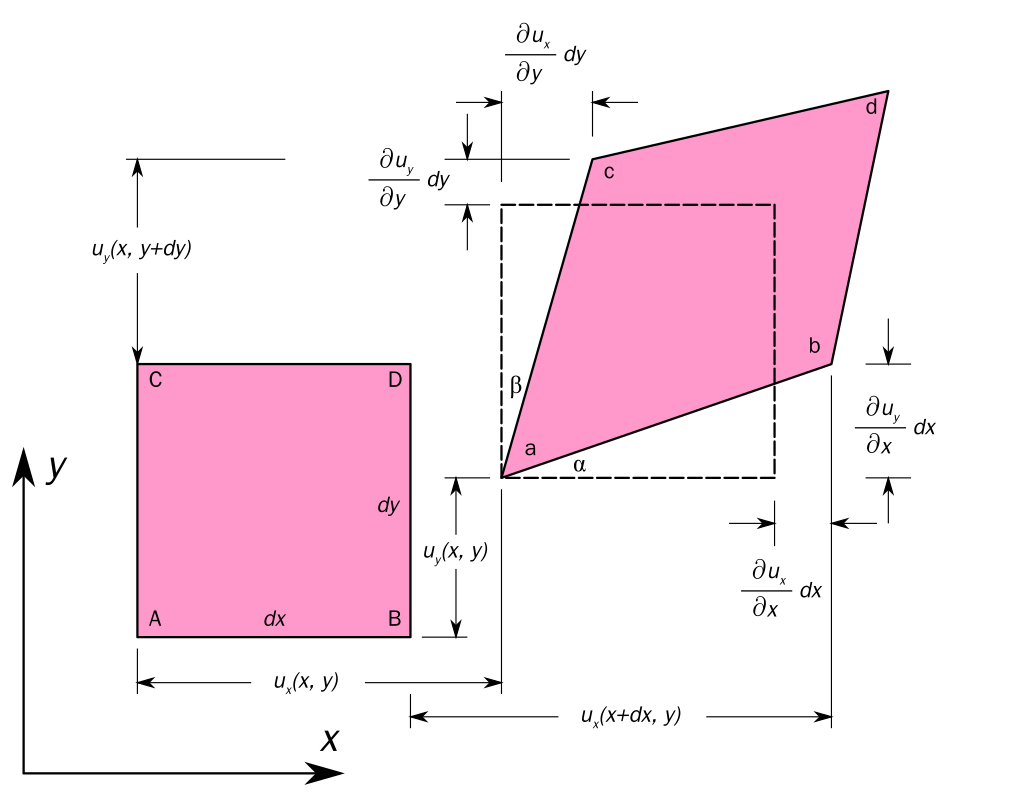
\includegraphics[width=0.8\textwidth]{figs/2D_geometric_strain.png}
    %\caption{Wikipedia}
\end{figure}

(Add the derivation of the book?)

\subsection{Macroscopic description}

Now that we know how the quantify strain, we can quantify the four main mechanical response,
    elastic,
    plastic,
    viscoelastic,
    and viscoplastic.
In a broad sense, the elastic relation is when the material returns to its original shape after load removal.
The plastic deformation is a permanent deformation once stress 


\paragraph{Elastic relation} The material returns to its original shape after load removal.
\begin{gather}
    \sigma_{ij} = C_{ijkl}\epsilon_{kl}
\end{gather}

\paragraph{Plastic relation} Deformation is permanent once stress exceeds a yield threshold.
\begin{gather}
    \sigma = \sigma_y \wedge \epsilon = \epsilon^e+\epsilon^p
\end{gather}

\paragraph{Viscoelastic relation} Time-dependent response combining elastic and viscous behaviour.
\begin{gather}
    \sigma + \lambda\dv{\sigma}{t} = E\epsilon+\eta\dv{\epsilon}{t}.
\end{gather}

\paragraph{Viscoplastic relation} Combines irreversible plastic strain with rate-dependent visvous effects
\begin{gather}
    \sigma = \sigma_y + \eta\dot{\epsilon}\mathrm{~for~}\sigma>\sigma_y
\end{gather}

\subsection{Microscopic description}


\paragraph{Stress} In continuum mechanics and physics, the measure of internal forces distributed within a material that arise in response to external loads is refered as stress.
As before, this measure is represented by a second-order tensor with units of \SI{}{\kilo\gram\per\meter\per\second\squared}.
The mathematical representation of the stress tensor is given by the Cauchy stress tensor, which relates a traction vector $\vec{T}$ acting on a surface $\vec{n}$ with the stress tensor $\bm{\sigma}$, equation~\eqref{eqn:stressTensor}.

\begin{figure}[ht!]
    \centering
    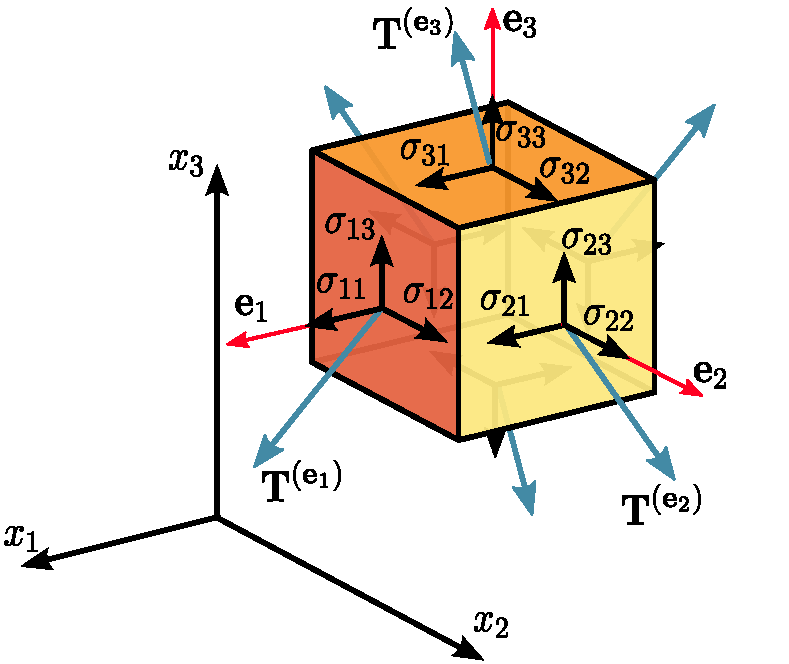
\includegraphics[width=0.8\textwidth]{figs/Components_stress_tensor_cartesian.pdf}
    %\caption{Wikipedia}
\end{figure}


\paragraph{Motivation: Molecular stress is equivalent to continuum stress} \dots This derivation can be found in the apendix of\citep{admalUnifiedInterpretationStress2010}\footnote{Describe more if what is done in this article}.\footnote{(Eventualmente pondré esto en párrafo) Notation:
    $\bm{\sigma}$ Tensor, $\vec{\sigma}$ vector, $\sigma_{i,j}$ tensor, $\overline{\sigma}$ time average, 
}
Consider a system of $N$ interacting particles with each particle position given by
\begin{equation}
    \vec{r}_{\alpha} = \vec{r} + \vec{s}_{\alpha}\label{eqn:DerVirTen1},
\end{equation}
where $\vec{r}$ is the position of the center of mass of the system and $\vec{s}_\alpha$ is the position of each point relative to the center of mass.
Hence, we can express the momentum of each particle as
\begin{equation}
    \vec{p}_\alpha = m_\alpha\qty(\dot{\vec{r}}+\dot{\vec{s}}_\alpha) = m_\alpha\qty(\dot{\vec{r}}+\vec{\upsilon}_\alpha^{\mathrm{rel}}).\label{eqn:DerVirTen2}
\end{equation}
Before starting the procedure, lets take into account that the center of mass of the system is given by
\begin{equation}
    \vec{r} = \frac{\sum_{\alpha}m_\alpha\vec{s}_\alpha}{\sum_{\alpha}m_\alpha}\label{eqn:DerVirTen3},
\end{equation}
and by replacing~\eqref{eqn:DerVirTen1} in~\eqref{eqn:DerVirTen2} we get the following relations, which will be used later,
\begin{equation}
    \sum_\alpha m_\alpha\vec{r}_\alpha = \vec{0},\quad
    \sum_\alpha m_\alpha\vec{\upsilon}_\alpha^{\mathrm{rel}} = \vec{0}.\label{eqn:DerVirTen4}
\end{equation}

Now we can start by computing the time derivative of tensorial product $\vec{r}_\alpha\otimes\vec{p}_\alpha$\footnote{It is interesting to note that the tensorial product $\vec{r}_\alpha\otimes\vec{p}_\alpha$ has units of action and by tacking the time derivative we are dealing with terms that has units of energy.
},
\begin{equation}
    \dv{t}\qty(\vec{r}_\alpha\otimes\vec{p}_\alpha) = 
    \underbrace{\vec{\upsilon}_\alpha^{\mathrm{rel}}\otimes\vec{p}_\alpha}_{\mathrm{Kinetic~term}} 
        +
        \underbrace{\vec{r}_\alpha\otimes\vec{f}_\alpha}_{\mathrm{Virial~term}},\label{eqn:DerVirTen5}
\end{equation}
which is known as the \textit{dynamical tensor virial theorem} and it is simply an alternative form to express the balance of linear momentum.
This theorem becomes useful after making the assumption that there existis a time scale $\tau$, which is short relative to macroscopic processes but long relative to the characteristic time of the particles in the system, over which the particles remain close to their original positions with bounded positions and velocities.
Taking advantage of this property we can compute the time average of~\eqref{eqn:DerVirTen5},
\begin{equation}
    \frac{1}{\tau}\qty(\vec{r}_\alpha\otimes\vec{p}_\alpha)\bigg|_{0}^{\tau} = 
    \overline{\vec{\upsilon}_\alpha^{\mathrm{rel}}\otimes\vec{p}_\alpha} 
        +
    \overline{\vec{r}_\alpha\otimes\vec{f}_\alpha}.\label{eqn:DerVirTen6}
\end{equation}
Assuming that $\vec{r}_\alpha\otimes\vec{p}_\alpha$ is bounded, and the time scales between microscopic and continuum processes are large enough, the term on the left-hand side can be as small as desired by tacking $\tau$ sufficiently large and by summing over all particles we achieve the \textit{tensor virial theorem}:
\begin{equation}
    \overline{\mathbf{W}} = -2\overline{\mathbf{T}},\label{eqn:DerVirTen7}
\end{equation}
where
\begin{equation}
    \overline{\mathbf{W}} = \sum_\alpha\overline{\vec{r}_\alpha\otimes\vec{f}_\alpha}\label{eqn:DerVirTen8}
\end{equation}
is the time-average virial tensor and
\begin{equation}
    \overline{\mathbf{T}}=\frac{1}{2}\sum_\alpha\overline{\vec{\upsilon}_\alpha^{\mathrm{rel}}\otimes\vec{p}_\alpha}\label{eqn:DerVirTen9}
\end{equation}
is the time-average kinetic tensor.
This expression for the tensor virial theorem applies equally to continuum systems that are not in macroscopic equilibrium as well as those that are at rest.

The assumption of the difference between the time scales allow us to simplify the relation by replacing~\eqref{eqn:DerVirTen2} in~\eqref{eqn:DerVirTen9}, so that,
\begin{equation}
    \overline{\mathbf{T}}=
        \frac{1}{2}\sum_\alpha m_\alpha\overline{\vec{\upsilon}_\alpha^{\mathrm{rel}}\otimes\vec{v}_\alpha^{\mathrm{rel}}}
        +
        \frac{1}{2} \left[\overline{\sum_\alpha m_\alpha\vec{\upsilon}_\alpha^{\mathrm{rel}}}\right]\otimes\dot{\vec{r}}\label{eqn:DerVirTen10},
\end{equation}
which is not the simplification we expected, however, by the relations from~\eqref{eqn:DerVirTen4}, equation~\eqref{eqn:DerVirTen10} simplifies to\footnote{No estoy muy seguro si incluir una discusión acerca del término cinético en la expresión del virial. Posiblemente un párrafo\dots posiblemente lo ponga en la interpretación del teorema.
También, no se si ir metiendo interpretación durante la derivación o no, pero bueno.}
\begin{equation}
    \overline{\mathbf{T}}=
        \frac{1}{2}\sum_\alpha m_\alpha\overline{\vec{\upsilon}_\alpha^{\mathrm{rel}}\otimes\vec{\upsilon}_\alpha^{\mathrm{rel}}}\label{eqn:DerVirTen11}.
\end{equation}
On the other hand, instead of reducing the expression, we start to create the conection with the Cauchy stress tensor by distributing~\eqref{eqn:DerVirTen8} into an internal and external contributions,
\begin{equation}
    \overline{\mathbf{W}} = 
    \underbrace{\sum_\alpha\overline{\vec{r}_\alpha\otimes\vec{f}_\alpha^{\mathrm{int}}}}_{\overline{\mathbf{W}}_{\mathrm{int}}}
        +
        \underbrace{\sum_\alpha\overline{\vec{r}_\alpha\otimes\vec{f}_\alpha^{\mathrm{ext}}}}_{\overline{\mathbf{W}}_{\mathrm{ext}}}.\label{eqn:DerVirTen12}
\end{equation}
The time-average internal virial tensor takes into account the interaction between particle $\alpha$ with the other particles in the system, meanwhile, the time-average external virial tensor considers the interaction with atoms outside the system, via a traction vector $\vec{t}$ and external fields acting on the system represented by $\rho\vec{b}$, where $\rho$ is the mass density of it and $\vec{b}$ is the body force per unit mass applied by the external field.
Therefore we can express the following,
\begin{equation}
    \sum_\alpha\overline{\vec{r}_\alpha\otimes\vec{f}_\alpha^{\mathrm{ext}}}
    :=
    \int_{\delta\Omega}\vec{\xi}\otimes\vec{t}dA 
    +
    \int_{\Omega}\vec{\xi}\otimes\rho\vec{b}dV.\label{eqn:DerVirTen13}
\end{equation}
Where $\vec{\xi}$ is a position vector within the domain $\Omega$ occupied by the system of particles with a continuous closed surface $\delta\Omega$.
Assuming that $\Omega$ is large enough to express the external forces acting on it in the form of the continuum traction vector $\vec{t}$.

With this we can substitute the traction vector with $\vec{t}=\bm{\sigma}\vec{n}$, where $\bm{\sigma}$ represent the Cauchy stress tensor and applying the divergence theorem in~\eqref{eqn:DerVirTen13}, we have 
\begin{equation}
    \overline{\mathbf{W}}_{\mathrm{ext}}
     =\int_{\Omega}
        \left[
            \vec{\xi}\otimes\rho\vec{b}+\mathrm{div}_{\vec{\xi}}\qty(\vec{\xi}\otimes\bm{\sigma})
        \right]dV
        =
    \int_{\Omega}
        \left[
            \bm{\sigma}^{\mathrm{T}}
            +
            \vec{\xi}\otimes\qty(\mathrm{div}_{\vec{\xi}}\bm{\sigma}+\rho\vec{b})
        \right]dV\label{eqn:DerVirTen14}
\end{equation}
Since we assume that we are under equilibrium conditions, the term $\mathrm{div}_{\vec{\xi}}\bm{\sigma}+\rho\vec{b}$ is zero~\eqref{eqn:DerVirTen14} it simplifies to
\begin{equation}
    \overline{\mathbf{W}}_{\mathrm{ext}}
    =V\bm{\sigma}^{\mathrm{T}}\label{eqn:DerVirTen15}.
\end{equation}
By tacking into account that we integrate over the domain $\Omega$ we can say that we compute the spatial average of the Cauchy stress tensor,
\begin{equation}
    \bm{\sigma}_{\mathrm{av}} =\frac{1}{V}\int_\Omega\bm{\sigma}dV\label{eqn:DerVirTen16},
\end{equation}
in which $V$ is the volume of the domain $\Omega$.
Replacing~\eqref{eqn:DerVirTen15} into~\eqref{eqn:DerVirTen12}, the tensor virial theorem~\eqref{eqn:DerVirTen7} can be expressed as,
\begin{equation}
    \sum_\alpha\overline{\vec{r}_\alpha\otimes\vec{f}_\alpha^{\mathrm{int}}}
    +
    V\bm{\sigma}_{\mathrm{av}}^{\mathrm{T}}
    =
    -\sum_\alpha m_\alpha\overline{\vec{\upsilon}_\alpha^{\mathrm{rel}}\otimes\vec{\upsilon}_\alpha^{\mathrm{rel}}}.\label{eqn:DerVirTen17}
\end{equation}
Finally, solving for the Cauchy Stress tensor we get,
\begin{equation}
    \bm{\sigma}_{\mathrm{av}}
    =
    -\frac{1}{V}
    \left[
        \sum_\alpha\overline{\vec{f}_\alpha^{\mathrm{int}}\otimes\vec{r}_\alpha}
        +
        \sum_\alpha m_\alpha\overline{\vec{\upsilon}_\alpha^{\mathrm{rel}}\otimes\vec{\upsilon}_\alpha^{\mathrm{rel}}}
    \right],\label{eqn:DerVirTen18}
\end{equation}
an expression that describe the macroscopic stress tensor in terms of microscopic variables\footnote{It is important to acknowledge that several mathematical subtleties were not taken into consideration, however all the mathematical formality is adressed by Nikhil Chandra Admal and E. B. Tadmor in~\citep{admalUnifiedInterpretationStress2010}}.

To end the section it is important to show that~\eqref{eqn:DerVirTen18} is symmetric.
Therefore, we rewrite the internal force as the sum of forces between the particles,
\begin{equation}
    \vec{f}^{\mathrm{int}}_\alpha = \sum_{{\beta}_{\beta\neq\alpha}}\vec{f}_{\alpha\beta}\label{eqn:DerVirTen19},
\end{equation}
and substituting~\eqref{eqn:DerVirTen19} into~\eqref{eqn:DerVirTen18}, we have
\begin{equation}
    \bm{\sigma}_{\mathrm{av}}
    =
    -\frac{1}{V}
    \left[
        \sum_{{\alpha,\beta}_{\beta\neq\alpha}}\overline{\vec{f}_{\alpha\beta}\otimes\vec{r}_\alpha}
        +
        \sum_\alpha m_\alpha\overline{\vec{\upsilon}_\alpha^{\mathrm{rel}}\otimes\vec{\upsilon}_\alpha^{\mathrm{rel}}}
    \right].\label{eqn:DerVirTen20}
\end{equation}
Due to the property $\vec{f}_{\alpha\beta}=-\vec{f}_{\beta\alpha}$ we obtain the following identity
\begin{equation}
    \sum_{{\alpha,\beta}_{\beta\neq\alpha}}\vec{f}_{\alpha\beta}\otimes\vec{r}_\alpha 
    =
    \frac{1}{2}\sum_{{\alpha,\beta}_{\beta\neq\alpha}}\left(\vec{f}_{\alpha\beta}\otimes\vec{r}_\alpha+\vec{f}_{\beta\alpha}\otimes\vec{r}_\beta\right)
    =
    \frac{1}{2}\sum_{{\alpha,\beta}_{\beta\neq\alpha}}\vec{f}_{\alpha\beta}\otimes\left(\vec{r}_\alpha-\vec{r}_\beta\right).\label{eqn:DerVirTen21}
\end{equation}
Therefore, by replacing the identity of~\eqref{eqn:DerVirTen21} into~\eqref{eqn:DerVirTen20}, we have
\begin{equation}
    \bm{\sigma}_{\mathrm{av}}
    =
    -\frac{1}{V}
    \left[
        \frac{1}{2}
        \sum_{{\alpha,\beta}_{\beta\neq\alpha}}\overline{\vec{f}_{\alpha\beta}\otimes\left(\vec{r}_\alpha-\vec{r}_\beta\right)}
        +
        \sum_\alpha m_\alpha\overline{\vec{\upsilon}_\alpha^{\mathrm{rel}}\otimes\vec{\upsilon}_\alpha^{\mathrm{rel}}}
    \right],\label{eqn:DerVirTen22}
\end{equation}
expressed with indexical notation and using the eistein summation convention,
\begin{equation}
    \sigma^{\mathrm{av}}_{ij}
    =
    -\frac{1}{V}
    \left[
        \frac{1}{2}
        \sum_{{\alpha,\beta}_{\beta\neq\alpha}}\overline{f^{\alpha\beta}_{i}r^\alpha_{j} + f^{\beta\alpha}_{i}r^\beta_{j}}
        +
        \sum_\alpha m_\alpha\overline{\upsilon^{\alpha~\mathrm{rel}}_{i}\upsilon^{\alpha{\mathrm{rel}}}_j}
    \right],\label{eqn:DerVirTen23}
\end{equation}
which is the same expression implemented in~LAMMPS\citep{LAMMPS}.\footnote{No se si poner la referencia a la pagina de documentacion\href{https://docs.lammps.org/compute_stress_atom.html}{https://docs.lammps.org/compute\_stress\_atom.html}}

\section{Molecular dynamics}

\paragraph{Intro} Here is the intro

\subsection{Langevin dynamics}

From a general point of view there are two types of methods to make a quatitative description of systems: one focused on simulating dynamics at the microscale, and the other dedicated to deriving or establishing evolutionary equations at the macroscale\citep{wangMultiscaleModelingSimulation2025}.
Since the assumption is made that the mechanical response of a hydrogel is predominantly derived from its internal structure\footnote{Poner citas que desmuestrén que no es hipótesis, si no que se sabe} we choose to simulate the dynamics at the microscale.
Additionally, by treating the hyrogel as a colloid, permits applying molecular dynamics to model its response under shear deformation. 
Finally, there are two commonly used mathematical frameworks to model the molecular dynamics, the continuous time random walk (CTRW) model and the Langevin equation\citep{wangMultiscaleModelingSimulation2025}, in this work we decided\footnote{Supongo que eventualmente justificaré la desición.} to use the langevin dynamics mathematical framework.

This is because, the solid phase of the colloid has a large mass and will change their momenta after many collisions with the solvent molecules and the picture which emerges is that of the heavy particles forming a system with a much longer time scale than the solvent molecules\citep{Thijssen2007} and Langevin theory takes advantage of this difference in time scale to eliminate the details of the degrees of freedom of the solvent particles and represent their effect by stochastic and dissipative forces allowing longer simulations that would be impossible if the solvent were explicitly included\citep{pastorTechniquesApplicationsLangevin1994}.
However, the representation of the solvent by a stochastic and dissipative force, introduce the problem of characterize two very different timescales, one associated with the slow relaxation of the initial velocity of the brownian particle and another linked to the frequent collisions that the brownian particle suffers with particles of the bath\citep{tsl2006}\footnote{Para traer a colación la sensibilidad de la respuesta mecánica al parámetro de damp.}. 
Therefore, two terms are used to create a mathematical representation of the solvent: a frictional force proportional to the velocity of the particle and a fluctuating force. 
Hence,
\begin{gather}
    m\dv{\vec{v}(t)}{t}=\vec{F}(t)-m\gamma\vec{v}(t)+\vec{R}(t).\label{eqn:BrownianDyn1}
\end{gather}
The friction constant $\gamma$\footnote{Cuidado con las unidades. Hacer análisis dimensional, porque por la condición de correlación en $R$, $\gamma$ ocupa tener unidades de masa entre tiempo, pero en la ecuación, solo ocupa unidades de $1/s$.} parametrises the effect of solvent damping and activation and is commonly referred to as the collision frequency in the simulation literature, even though formally a Langevin description implies that the solute suffers an infinite number of collisions with infinitesimally small momentum transfer.
Also, the fact that the second term is not a function of the position of any of the particles involves the neglect of hydrodynamic interaction or spatial correlation in the friction kernel spatial correlation in the friction kernel\citep{pastorTechniquesApplicationsLangevin1994}.
On the other hand, $\vec{R}(t)$\footnote{No me acuerdo en donde está que se puede asumir que tiene distribución gaussiana.} is a ``random force'' subject to the following conditions
\begin{align*}
    \expval{\vec{R}(t)} &= 0 \\
    \expval{\vec{R}(t)\vec{R}(t')} &= 2k_{B}T\gamma\delta\qty(t-t') 
\end{align*}
The no time correlation is equivalent to assuming that the viscoelastic relaxation of the solvent is very rapid with respect to solute motions\footnote{Grote land Hynes [26] have investigated this assumption for motions involving barrier crossing and have found that while it is seriously in error for passage over sharp barriers (such as 12 recombination); it is quite adequate for conformational transitions such as might be found in polymer motions.\citep{pastorTechniquesApplicationsLangevin1994}}.

In comparing the results of Langevin dynamics with those of other stochastic methods [28-31], the relevant variable is the velocity relaxation time, $\tau_{v}$ which equals $\gamma^{-1}$\citep{pastorTechniquesApplicationsLangevin1994}
The Langevin equation improves conformational sampling over standard molecular dynamics\citep{paquetMolecularDynamicsMonte2015}.

\begin{itemize}
    \item Hablar acerca de que la fuerza aleatoria puede tener distribución gaussiana, pero no necesariamente.
    \item hablar de la ecuación de Green-Kubo: \[\eta=\frac{V}{k_B T}\int_{0}^{\infty}\expval{\sigma_{xy}(t)\sigma_{xy}(0)}\mathrm{d}t\]
    \item No se que tanto hablar de la idea de correlación y su aplicación en estos temas.
\end{itemize}

\subsection{Velocity Verlet}

\paragraph{Intro} The core concept of the Velocity Verlet algorithm is to update particle positions and velocities using both current and predicted accelerations, ensuring time-reversibility and energy conservation over long simulations. 
In systems governed by Langevin dynamics, the algorithm can incorporate random forces consistent with the fluctuation-dissipation theorem to simulate physically realistic Brownian motion.

From a mathematical point of view, this algorithm is a second-order integratos for ordinary differential equations.
Furthermore, from a computational perspective, Velocity Verlet is an explicit algorithm, easy to implement, and efficient in term of memory usage.
It requires only the positions, velocities, and accelerations from the previous timestep.
Which allows efficient parallelization and eliminates the need for additional memory allocations per step.


